% HUMAN_REPRODUCTION_V6_2026_10_30
\documentclass[11pt,a4paper]{article}
\usepackage[margin=25mm]{geometry}
\usepackage[T1]{fontenc}
\usepackage{mathpazo,amsmath,amssymb,graphicx,booktabs,longtable,array,caption,setspace,microtype}
\usepackage[authoryear,round]{natbib}
\usepackage[hidelinks]{hyperref}
\usepackage{fancyhdr}
\usepackage{placeins}
\usepackage[mathlines]{lineno}
\doublespacing
\setlength{\parskip}{4pt}
\setlength{\parindent}{0pt}
\captionsetup{font=small,labelfont=bf}
\pagestyle{fancy}\fancyhf{}\fancyhead[L]{\small PCOS infertility and reference composition}\fancyhead[R]{\thepage}
\setlength{\headheight}{14pt}
\setlength{\emergencystretch}{2em}
\newcommand{\ASPR}{\mathrm{ASPR}}
\title{Reference-country composition and age-standardized PCOS-attributed infertility contrasts: China and 18 G20 countries, 1990--2023}
\author{XX Author$^{1}$, XX Author$^{2}$, XX Corresponding Author$^{1,*}$\\
{\small $^{1}$XX Department, XX Institution, XX City, XX Country, XX Postal code}\\
{\small $^{2}$XX Department, XX Institution, XX City, XX Country, XX Postal code}\\
{\small $^{*}$Correspondence: XX email; ORCID: XX}}
\date{30 October 2026}

\begin{document}
\maketitle\thispagestyle{fancy}
\noindent\textbf{Running title:} PCOS infertility and reference composition

\linenumbers
\begingroup\sloppy
\begin{abstract}
\noindent\textbf{STUDY QUESTION:} How did changing reference-country population shares contribute to China's PCOS-attributed infertility rate difference from an 18-country pool during 1990--2023?

\noindent\textbf{SUMMARY ANSWER:} Reference-country composition contributed +88.65 per 100,000 females to the +151.54 change in the modeled difference, or 58.5\% of its signed net change.

\noindent\textbf{WHAT IS KNOWN ALREADY:} GBD studies describe PCOS-attributed infertility burden and trends. Fixed age-standardization weights still permit country composition within each reference age group to change.

\noindent\textbf{STUDY DESIGN, SIZE, DURATION:} This exploratory ecological analysis covered China and 18 other sovereign G20 countries, females aged 15--49 in seven age groups, and 34 years, 1990--2023.

\noindent\textbf{PARTICIPANTS/MATERIALS, SETTING, METHODS:} GBD 2023 prevalence counts and matched female populations yielded age-specific rates. Fixed age weights were normalized over ages 15--49. The primary estimand was the change in China's total-infertility standardized rate difference from the contemporaneous population-pooled reference. Symmetric accounting separated Chinese rates, reference-country rates and reference-country shares. UN WPP 2024 replaced shares only; subtypes and alternative benchmarks addressed secondary questions. Sensitivity analyses covered country exclusions, age restriction, alternative endpoints, annual chaining and all 128 rounding-perturbation corners of published age weights.

\noindent\textbf{MAIN RESULTS AND THE ROLE OF CHANCE:} China's total rate rose from 333.56 to 605.08 and the reference rate from 606.48 to 726.45 per 100,000. Their difference narrowed from $-272.92$ to $-121.38$. The respective rate and composition components were $+271.51-208.62+88.65=+151.54$ (rounded). UN shares gave +86.76 for composition and +150.69 overall. The 2023 secondary-infertility difference was +2.16 with contemporaneous GBD shares, $-47.99$ with fixed-1990 shares and $-127.89$ with equal-country weights. Results are derived point estimates; jointly aligned posterior draws were not obtained for interval propagation.

\noindent\textbf{LIMITATIONS, REASONS FOR CAUTION:} Uncertainty in component magnitudes and near-zero contrast signs remains unquantified. The signed net denominator contains opposing components, so 58.5\% is an accounting ratio. Rounded published age weights and the economically selected G20 reference also limit interpretation.

\noindent\textbf{WIDER IMPLICATIONS OF THE FINDINGS:} Reproductive-health monitoring against pooled populations should report reference weights and absolute components alongside net differences. Doing so distinguishes changes in national rates from changes in the population represented by the benchmark.

\noindent\textbf{FUNDING:} XX: verified funding sources and funder roles to be completed by the authors at submission.

\noindent\textbf{DISCLOSURES:} XX: author-specific disclosures to be completed at submission.

\noindent\textbf{TRIAL REGISTRATION NUMBER:} Not applicable; this is a secondary analysis of aggregate estimates, not a clinical trial.
\end{abstract}
\endgroup

\textbf{Keywords:} Polycystic Ovary Syndrome; Infertility, Female; Prevalence; Age Distribution; Population Dynamics.

\section{Introduction}
Polycystic ovary syndrome (PCOS) affects reproductive health and requires care tailored to the individual \citep{pcos}. Population monitoring complements this clinical perspective by describing national trajectories in PCOS-attributed infertility. In the Global Burden of Disease (GBD) study, this outcome is a modeled cause-specific infertility impairment expressed in the general female population \citep{gbd}. Interpreting a national trajectory against a pooled international population requires an explicit definition of that reference.

Liu and colleagues quantified GBD 2019 PCOS-attributed infertility prevalence, disability and geographical trends \citep{liu_pcos2024}. Liang and colleagues analysed GBD 2021 burden, trends and the contributions of population growth, ageing and epidemiological change to burden counts \citep{liang_burden2025}; another study examined China and worldwide trajectories \citep{liang_trend2026}. These studies establish the burden context. Our question concerns the construction of a particular national-versus-pool rate contrast, with country shares changing within age even when the age standard remains fixed (Supplementary Table~S9).

A contemporaneous population pool represents the country mix at each date. If countries with lower age-specific rates gain population share, the pooled rate can fall even with unchanged country-specific rates. This composition term operates within age and therefore persists after age standardization. We quantified the 1990--2023 change in China's total PCOS-attributed infertility rate difference from the population-pooled reference of 18 other sovereign G20 countries, allocating that change to Chinese rates, reference-country rates and reference-country shares. Secondary questions concern demographic-source choice, infertility subtypes and fixed-1990 or equal-country benchmarks.

\section{Materials and methods}
\subsection{Design data and outcome}
This ecological secondary analysis used GBD 2023 Results Tool exports obtained on 25 October 2026 \citep{results}. We analysed females aged 15--49 in seven five-year age groups during 1990--2023. The fixed set comprised 19 sovereign G20 countries, with China excluded from the reference. The 18 reference countries were Argentina, Australia, Brazil, Canada, France, Germany, India, Indonesia, Italy, Japan, Republic of Korea, Mexico, Russian Federation, Saudi Arabia, South Africa, T\"urkiye, United Kingdom and United States of America. The G20 was established in 1999; we applied this country set retrospectively across the study years. The European Union and African Union were excluded as additional units to avoid overlapping country populations \citep{g20}.

We selected prevalence (measure 5), PCOS (cause 605), total infertility (impairment 198), primary infertility (220) and secondary infertility (221). Endometriosis (607) was retained as a supplementary comparator. The GBD 2023 household-survey framework identifies primary infertility using absence of a livebirth, desire for a child, union duration of at least five years and no current contraception. Its secondary definition requires a livebirth more than five years earlier and the corresponding union, fertility-intention and contraception conditions. The modeling process combines these survey envelopes with sex- and cause-attribution evidence, including clinical sources, and expresses the final rates among all females in each age group \citep{gbd}. Supplementary data distinguish these quantities from clinical 12-month infertility definitions and from PCOS prevalence itself.

For country $c$, age $a$, year $t$ and infertility type $k$, let $N_{c,a,t,k}$ denote modeled infertility cases and $P_{c,a,t}$ the matched GBD female population. Age-specific prevalence per 100,000 is $r_{c,a,t,k}=10^5N_{c,a,t,k}/P_{c,a,t}$. We checked unique complete cells, finite nonnegative values, primary-plus-secondary additivity and agreement with separately exported endpoint Rate values. Input specifications and hashes are retained in the reproducibility archive.

\subsection{Annual contrasts and the primary period change}
Let $\mathcal{R}$ be the set of 18 reference countries; the labels $\mathrm{CHN}$ and $\mathrm{R}$ denote China and the pooled reference. We normalized the seven published age weights over ages 15--49 and held them fixed. Their six-decimal reproduction is attributed to Chen and colleagues \citep{chen}; an official full-precision IHME vector was not independently verified.
\begin{align}
 s_{c,a,t}&=\frac{P_{c,a,t}}{\sum_{j\in\mathcal{R}}P_{j,a,t}}, &
 A_{\mathrm{R},t,k}&=\sum_a w_a\sum_{c\in\mathcal{R}}s_{c,a,t}r_{c,a,t,k},\\
 A_{\mathrm{CHN},t,k}&=\sum_a w_ar_{\mathrm{CHN},a,t,k}, &
 D_{t,k}&=A_{\mathrm{CHN},t,k}-A_{\mathrm{R},t,k}.
\end{align}
Here $w_a$ sums to one, and $s_{c,a,t}$ sums to one over reference countries within each age and year. Pooling within age precedes standardization. The annual rate difference is $D_{t,k}$; its period change is $\Delta D_k(t_0,t_1)=D_{t_1,k}-D_{t_0,k}$. The primary estimand is $\Delta D_{\mathrm{total}}(1990,2023)$ under contemporaneous GBD shares. Subtype and alternative-reference analyses address secondary estimands. All rates are restricted-age standardized rates per 100,000 females.

\subsection{Symmetric decomposition of the period change}
For endpoints $t_0$ and $t_1$, the symmetric product identity of Kitagawa-type accounting gives \citep{kitagawa}:
\begin{align}
 \Delta D_k(t_0,t_1)&=X_k+Q_k+S_k,\\
 X_k&=\sum_a w_a(r_{\mathrm{CHN},a,t_1,k}-r_{\mathrm{CHN},a,t_0,k}),\\
 Q_k&=-\sum_a w_a\sum_{c\in\mathcal{R}}\frac{s_{c,a,t_0}+s_{c,a,t_1}}{2}(r_{c,a,t_1,k}-r_{c,a,t_0,k}),\\
 S_k&=-\sum_a w_a\sum_{c\in\mathcal{R}}\frac{r_{c,a,t_0,k}+r_{c,a,t_1,k}}{2}(s_{c,a,t_1}-s_{c,a,t_0}).
\end{align}
$X_k$, $Q_k$ and $S_k$ allocate the period change to Chinese rates, reference-country rates and reference-country shares, respectively. Each uses the same endpoints, subtype and population-source specification. Averaging the two replacement orders splits the product interaction symmetrically, giving an exact identity before rounding. Positive components raise the signed China-minus-reference difference. When the difference is negative, an upward change narrows it.

The identity is additive across ages and types. The share component is zero if shares are unchanged; it also vanishes when the countries' mean endpoint rates are identical within age, because share changes sum to zero. These algebraic properties clarify the role of composition. Its estimated magnitude in the GBD data is reported separately below.

We report absolute components before the ratio $100S_k/\Delta D_k(t_0,t_1)$. Its signed net denominator contains cancellation between components and can approach zero; ratios can consequently exceed 100\% or change sign. This accounting ratio is distinct from a fraction of women, cases or disease causation. Subtype and country-share contributions partition the same change in different ways and are not additive explanations.

\subsection{Population sources and benchmark definitions}
UN WPP 2024 supplied historical mid-year female population estimates for the same 4,522 country--age--year cells \citep{wpp2024}. Values in thousands were converted to persons; projections from 2024 onward were excluded. Only the within-age reference shares were replaced. GBD cases continued to use matched GBD population denominators, and the age standard remained fixed.

Current-year shares compare China with the contemporaneous pooled population. Fixed-1990 shares hold the reference's 1990 within-age country mix constant while country rates vary. Equal-country weights compare China with the arithmetic mean of 18 country rates within age. These benchmarks specify different reference populations and therefore different descriptive estimands. A fixed-share path is distinct from the symmetric share component.

\subsection{Structural sensitivity and posterior uncertainty}
Existing sensitivity analyses used both population sources, each country exclusion, ages 20--49 with renormalized weights, 1990 or 2010 start years, and 2021, 2022 or 2023 endpoints. Adjacent-year decompositions were summed over 1990--2023. All $2^7=128$ perturbation corners of the unnormalized age weights by $\pm0.5\times10^{-6}$ assessed rounding. These are scenario and numerical-precision checks. Supplementary endometriosis analyses include all annual subtype differences and recent endpoint comparisons, supporting descriptive examination of cancellation \citep{xu}.

The available study exports contain marginal summaries without posterior draw columns. The documented access audit did not identify a provider-confirmed joint array aligned across countries, ages, years and infertility types. Derived results therefore remain point estimates without propagated uncertainty intervals or significance tests. Marginal bounds, independent simulation and country bootstrap do not recover the required joint dependence. Eligible draws would require provider alignment evidence and product-summary checks before recomputing pooling and decomposition within each draw. Ratios would additionally require diagnostics for a near-zero net-change denominator.

\subsection{Computational reproducibility}
The exploratory analyses were not externally preregistered. Core results were independently calculated in Python 3.12.14 and base R 4.6.1. The recorded Python scientific environment used NumPy 2.3.5, pandas 2.2.3 and Matplotlib 3.10.7. These are external libraries, separate from the language's standard library. The source manifest, code and aggregate results are pinned to the immutable research snapshot \citep{repository}. The supplement provides the code-variable notation map, commands, numerical checks and GATHER reporting map \citep{gather}.

\subsection{Ethical approval}
Public aggregate GBD estimates and UN demographic data were analysed without individual participant records. XX: institutional ethics-review applicability or exemption determination to be confirmed by the responsible author. No ethics approval number is asserted.

\subsection{Use of artificial intelligence}
OpenAI ChatGPT and Codex supported code development, analysis checks, drafting and technical editing, including this revision on 30 October 2026. Acknowledgements records the verified earlier model identifier, version limits and pending author-review status.

\section{Results}
\subsection{Coverage and PCOS contrasts}
The GBD population and UN subset each covered 4,522 cells. The prevalence analysis contained 27,132 country--age--year--cause--type cells across the two causes, including 13,566 PCOS cells. Completeness, subtype additivity, endpoint rate reconstruction and independent R/Python checks passed; numerical details are in Supplementary data.

China's PCOS-attributed total infertility standardized rate increased from 333.56 to 605.08 per 100,000, while the population-pooled reference increased from 606.48 to 726.45 (Table~\ref{tab:pcos}; Figure~\ref{fig:trends}). The difference changed from $-272.92$ to $-121.38$ and the ratio from 0.550 to 0.833. The narrower negative difference therefore accompanied increases in both standardized rates.

\begin{table}[htbp]\centering\small\setstretch{1.15}
\caption{PCOS-attributed infertility rates and contrasts under contemporary GBD population shares.}\label{tab:pcos}
\begin{tabular}{llrrrr}\toprule
Type & Year & China & Reference & Difference & Ratio\\\midrule
Total & 1990 & 333.56 & 606.48 & -272.92 & 0.550\\
Total & 2023 & 605.08 & 726.45 & -121.38 & 0.833\\
Primary & 1990 & 44.70 & 214.64 & -169.94 & 0.208\\
Primary & 2023 & 97.35 & 220.89 & -123.54 & 0.441\\
Secondary & 1990 & 288.86 & 391.84 & -102.98 & 0.737\\
Secondary & 2023 & 507.72 & 505.56 & +2.16 & 1.004\\
\bottomrule
\end{tabular}
\caption*{Rates and differences are per 100,000 females, standardized within ages 15--49. Difference is China minus reference. All are model point estimates without propagated posterior intervals.}
\end{table}

\subsection{Absolute decomposition before percentages}
The 1990--2023 change in the total contrast was
\begin{equation}
 \underbrace{+271.51}_{X}\;\underbrace{-208.62}_{Q}\;\underbrace{+88.65}_{S}
 =\underbrace{+151.54}_{\Delta D}\quad\text{per 100,000},
\end{equation}
with displayed rounding (Table~\ref{tab:decomp}; Figure~\ref{fig:decomp}). Chinese rate changes and reference-share changes moved the signed difference upward, while reference-country rate changes offset them. The country-share term was 58.5\% of the signed net change; this denominator is smaller because positive and negative terms cancel.

The country-share component was +88.11 ending in 2021 and +86.74 ending in 2022. The annual-chained component was +87.11 (57.5\%). Across 18 country exclusions and restriction to ages 20--49, the GBD 1990--2023 country-share ratio ranged from 39.8\% to 67.9\% (Supplementary data, Table~S2 and Figure~S3). The contribution persisted across these specifications, with its ratio to the net change varying with the age range and reference countries.

Secondary infertility contributed +105.14 and primary infertility +46.40 to the +151.54 total change. The secondary contribution was 69.4\% of the signed net change. Its country-share component was +56.81, compared with +31.84 for primary infertility. These ratios describe intersecting partitions of the same total change, as defined in Methods.

\begin{table}[htbp]\centering\small\setstretch{1.15}
\caption{Symmetric PCOS contrast-change decomposition, 1990--2023, by population source.}\label{tab:decomp}
\setlength{\tabcolsep}{4pt}
\begin{tabular}{llrrrr}\toprule
Type & Shares & China rates $X$ & Ref. rates $Q$ & Ref. shares $S$ & Net $\Delta D$\\\midrule
Total & GBD & +271.51 & -208.62 & +88.65 & +151.54\\
Total & UN WPP & +271.51 & -207.59 & +86.76 & +150.69\\
Primary & GBD & +52.65 & -38.09 & +31.84 & +46.40\\
Primary & UN WPP & +52.65 & -37.75 & +30.13 & +45.02\\
Secondary & GBD & +218.86 & -170.53 & +56.81 & +105.14\\
Secondary & UN WPP & +218.86 & -169.83 & +56.64 & +105.67\\
\bottomrule
\end{tabular}
\caption*{All contributions are per 100,000 females, with fixed standard age weights. Components sum before rounding. UN changes country shares only. Positive and negative components may cancel; percentages use the signed net denominator defined in Methods.}
\end{table}

\subsection{Population-source and benchmark sensitivity in the main results}
UN weighting gave a total contrast change of +150.69, decomposed as +271.51 from Chinese rates, $-207.59$ from reference rates and +86.76 from country shares (57.6\%; Figure~\ref{fig:source}). The 2023 total difference was $-122.62$, compared with $-121.38$ under GBD shares. Mean total-variation distance between the two within-age reference-share vectors was 1.32 percentage points in 2023 and 1.13 over all years. The share and net-change components were close under the two population sources.

Under current GBD shares, the 2023 primary PCOS difference was $-123.54$, while the secondary difference was +2.16 (Figure~\ref{fig:subtypes}). With UN shares the secondary difference was +2.26, but fixing UN shares at 1990 changed it to $-48.34$; equal-country weighting changed it to $-127.89$ (Table~\ref{tab:bench}; Figure~\ref{fig:bench}). GBD fixed-1990 shares gave $-47.99$. The 2023 secondary point estimate was positive under contemporary shares and negative under both alternatives, demonstrating the dependence of this contrast on the reference definition.

\begin{table}[htbp]\centering\small\setstretch{1.15}
\caption{Benchmark definition changes the 2023 PCOS secondary infertility contrast.}\label{tab:bench}
\begin{tabular}{llrr}\toprule
Population source & Benchmark & Reference rate & China minus reference\\\midrule
GBD & Current-year shares & 505.56 & +2.16\\
GBD & Fixed-1990 shares & 555.71 & -47.99\\
GBD & Equal countries & 635.61 & -127.89\\
UN WPP & Current-year shares & 505.46 & +2.26\\
UN WPP & Fixed-1990 shares & 556.06 & -48.34\\
UN WPP & Equal countries & 635.61 & -127.89\\
\bottomrule
\end{tabular}
\caption*{China's standardized rate is 507.72 per 100,000 throughout. Country weights are applied within each age; the same GBD disease rates and age standard are used. Equal-country rows are identical by construction. Each row represents a different benchmark definition.}
\end{table}

\section{Discussion}
Reference-country composition made a substantial contribution to the narrowing PCOS-attributed infertility contrast between China and the pooled reference. With a fixed age standard, the 1990--2023 signed rate difference increased by +151.54 per 100,000: +271.51 from Chinese rates, $-208.62$ from reference-country rates and +88.65 from changing reference-country shares. The close +86.76 share component under UN populations supports stability to this demographic-source substitution. Both China's and the reference's total modeled rates rose, so the narrower contrast describes their relative trajectories alongside the changing population mix.

This analysis adds a reference-construction perspective to geographical burden and trend studies \citep{liu_pcos2024,liang_burden2025,liang_trend2026}. Holding age weights fixed retains variation in country shares within age. Explicit decomposition makes that source of change visible in the national-versus-pool comparison. Established symmetric accounting gives the absolute contributions in the same rate units as the observed difference. This application concerns an explicitly defined pool and period; the prior studies address the targets summarized in Supplementary Table~S9.

The practical implication is to specify the population represented by a benchmark and show its weights with the comparison. Contemporary pooling addresses the country mix at each date, fixed historical shares address a constant mix, and equal-country weighting gives small and large countries equal influence within age. The 2023 secondary-infertility point estimate is positive under contemporary shares and negative under the alternatives. Reporting these targets together reveals the benchmark dependence of that near-zero contrast. Absolute components should accompany ratios: the 58.5\% share ratio uses a net denominator reduced by opposing rate components, and its 39.8\%--67.9\% range across the specified age and country-exclusion scenarios describes sensitivity to those choices.

Clinical interpretation also depends on the outcome and denominator. Yang and colleagues' Chinese community survey used Rotterdam PCOS ascertainment among married Han women aged 20--49 and reported infertility characteristics among PCOS participants \citep{yang}. The present analysis instead concerns GBD cause-attributed infertility among all females aged 15--49. These definitions and populations serve different purposes (Supplementary Table~S11). The clinical guideline provides the diagnostic and care context \citep{pcos}; the aggregate comparison does not identify individual transitions between infertility categories or effects of diagnosis, treatment or service provision.

The principal limitation is unquantified joint posterior uncertainty. Without verified aligned draws, the precision of absolute components, the 58.5\% ratio and near-zero contrast signs remains unknown; scenario analyses cannot supply that precision. Additional limits include heterogeneous upstream evidence and modeled attribution, possible shared population inputs between GBD and UN, rounded published age weights, exploratory analytical choices and the economically selected country set. The results describe this G20 comparison rather than the world or a matched clinical control. The computational audits check implementation and source-output consistency, while clinical validity requires evidence matched to the modeled definitions.

Reproductive-health monitoring can be made more interpretable by reporting the signed national-versus-reference change together with absolute rate and country-composition components. In these estimates, the reference population's changing composition accounts for +88.65 per 100,000 of a +151.54 change, providing information that the net contrast alone would conceal.

\section*{Authors' roles}
XX: verified author-by-author contributions to design, execution, analysis, drafting and critical discussion, final approval and accountability to be supplied at submission.

\section*{Acknowledgements}
We acknowledge the GBD data providers and collaborators and the United Nations Population Division. XX: additional acknowledgements, if applicable.

OpenAI ChatGPT and Codex supported code development, analysis checks, drafting and technical editing under researcher-specified questions and revision instructions, including editorial revision and document checks on 30 October 2026. The earlier documented Codex session on 29 October 2026 recorded \texttt{gpt-6.1-sol}; exact model versions for earlier separate ChatGPT sessions and an independently verified serving identifier for this later revision are not specified. No artificial observations or posterior draws replaced study data. The authors' final scientific review, verification of AI-supported content and approval remain to be confirmed before submission; human authors retain responsibility for the work.

\section*{Funding}
XX: verified sponsors, grants and funder roles, or an author-approved no-specific-funding statement, to be supplied at submission.

\section*{Disclosures}
XX: author-specific financial, personal and professional disclosures to be supplied at submission.

\section*{Data availability}
The executable Python and R workflow, aggregate derived results, query specifications and checksums are available in the immutable public research snapshot \citep{repository}. The snapshot identifies the analysis underlying the present article and is distinct from the manuscript version. Licensed original GBD 2023 extracts were accessed through the GBD Results Tool on 25 October 2026 \citep{results}; the query dimensions, export identifiers and SHA-256 hashes needed to identify them are recorded in the snapshot's input manifest. These originals and country--age source-cell extracts are retained in the private research archive and are excluded from the public repository. UN WPP 2024 population data are identified by the exact source product and file in the reference list \citep{wpp2024}; the attributed 4,522-row subset and its source manifest are included in the immutable snapshot. No hospital data were used.

\section*{Supplementary data}
Supplementary methods, nine numerical tables (S1--S8 and S10), seven figures, the literature/estimand comparison (S9), the outcome-definition comparison (S11), and a GATHER reporting map accompany the article. A complete annual subtype CSV and dated source, notation and revision audits are included in the reproducibility archive. The reproducibility archive contains code, aggregate results, source specifications and a README; licensed GBD originals and restricted source cells are excluded.

{\small\setstretch{1.2}
\begin{thebibliography}{99}
\bibitem[Australian Government(2026)]{g20}Australian Government Department of Foreign Affairs and Trade. The G20. Accessed 30 October 2026. \url{https://www.dfat.gov.au/trade/organisations/g20}.

\bibitem[Chen et al.(2026)]{chen}Chen S, Yang X, Jiang S, Lin Y, Huang L, Chen H, Zheng J, Xie Y, Kuang Z. Burden and temporal trends of female-specific cancers in China: a systematic analysis of the 2023 global burden of disease study. \emph{PLOS One}. 2026;21:e0351539. Supplemental table of reproduced GBD standard population. \href{https://doi.org/10.1371/journal.pone.0351539}{doi:10.1371/journal.pone.0351539}.
\bibitem[GBD 2023 Collaborators(2025)]{gbd}GBD 2023 Disease and Injury and Risk Factor Collaborators. Burden of 375 diseases and injuries, risk-attributable burden of 88 risk factors, and healthy life expectancy in 204 countries and territories, including 660 subnational locations, 1990--2023: a systematic analysis for the Global Burden of Disease Study 2023. \emph{Lancet}. 2025;406(10513):1873--1922. \href{https://doi.org/10.1016/S0140-6736(25)01637-X}{doi:10.1016/S0140-6736(25)01637-X}. Includes Supplementary Appendix 1, infertility methods.
\bibitem[Institute for Health Metrics and Evaluation(2026)]{results}[dataset] Institute for Health Metrics and Evaluation. GBD 2023 prevalence and matched female-population extracts for China and 18 other G20 countries, 1990--2023. GBD Results Tool; extracts accessed 25 October 2026. \url{https://vizhub.healthdata.org/gbd-results/}. Release: GBD 2023; export identifiers 1b13e337, 916826fb, 416daf73 and 76c5523c. Query specifications and input hashes are provided in the versioned research snapshot listed below. Access is subject to IHME terms.
\bibitem[Kitagawa(1955)]{kitagawa}Kitagawa EM. Components of a difference between two rates. \emph{J Am Stat Assoc}. 1955;50(272):1168--1194. \href{https://doi.org/10.1080/01621459.1955.10501299}{doi:10.1080/01621459.1955.10501299}.
\bibitem[Liang(2026)]{liang_trend2026}Liang Q. Trend analysis of the burden of PCOS and related infertility in China and worldwide between 1990 and 2021. \emph{Reprod Biomed Online}. 2026;52(2):105239. Published online 2 September 2025. \href{https://doi.org/10.1016/j.rbmo.2025.105239}{doi:10.1016/j.rbmo.2025.105239}.
\bibitem[Liang et al.(2025)]{liang_burden2025}Liang Y, Zhong K, Huang Z, Shi W, Ou Y. Global, regional, and national burden of infertility attributable to polycystic ovary syndrome, 1990--2021: results from the Global Burden of Disease Study 2021. \emph{Front Public Health}. 2025;13:1693486. \href{https://doi.org/10.3389/fpubh.2025.1693486}{doi:10.3389/fpubh.2025.1693486}.
\bibitem[Liu et al.(2024)]{liu_pcos2024}Liu X, Zhang J, Wang S. Global, regional, and national burden of infertility attributable to PCOS, 1990--2019. \emph{Hum Reprod}. 2024;39:108--118. \href{https://doi.org/10.1093/humrep/dead241}{doi:10.1093/humrep/dead241}.
\bibitem[PCOS research workspace(2026)]{repository}[dataset] PCOS research workspace. Analysis code, query manifests and aggregate derived results for GBD 2023 infertility comparisons. GitHub; 2026. Immutable revision 1abf337d9f23cc69292e03cd581b6a1557e6effe. \url{https://github.com/jiabao1314/PCOS/tree/1abf337d9f23cc69292e03cd581b6a1557e6effe/PCOS_Revision_2026-10-29}. Includes the Python/R workflow, input manifest, aggregate results and attributed UN population subset; restricted GBD originals are excluded.
\bibitem[Stevens et al.(2016)]{gather}Stevens GA, Alkema L, Black RE, Boerma JT, Collins GS, Ezzati M, Grove JT, Hogan DR, Hogan MC, Horton R, et al. Guidelines for Accurate and Transparent Health Estimates Reporting: the GATHER statement. \emph{PLOS Med}. 2016;13:e1002056. \href{https://doi.org/10.1371/journal.pmed.1002056}{doi:10.1371/journal.pmed.1002056}.
\bibitem[Teede et al.(2023)]{pcos}Teede HJ, Tay CT, Laven JJE, Dokras A, Moran LJ, Piltonen TT, Costello MF, Boivin J, Redman LM, Boyle JA, et al. Recommendations from the 2023 International Evidence-based Guideline for the Assessment and Management of Polycystic Ovary Syndrome. \emph{J Clin Endocrinol Metab}. 2023;108:2447--2469. \href{https://doi.org/10.1210/clinem/dgad463}{doi:10.1210/clinem/dgad463}.
\bibitem[United Nations(2024)]{wpp2024}[dataset] United Nations, Department of Economic and Social Affairs, Population Division. World Population Prospects 2024, Online Edition: population by five-year age group and sex, medium variant, midyear. United Nations; 2024. Source file: \texttt{WPP2024\_PopulationByAge5GroupSex\_Medium.csv.gz}. \url{https://population.un.org/wpp/assets/Excel%20Files/1_Indicator%20(Standard)/CSV_FILES/WPP2024_PopulationByAge5GroupSex_Medium.csv.gz}. Historical estimates through 2023 only were selected. Creative Commons Attribution 3.0 IGO.
\bibitem[Xu et al.(2025)]{xu}Xu Y, Jia Y, Li Q, Jiang H, Xiong Y, Liang W, Liu X, Huang Y, Zou K, Sun X, et al. Global, regional, and national burden of endometriosis, PCOS, and unexplained infertility and their attribution to infertility, 1990--2021: Global Burden of Disease Study 2021. \emph{J Evid Based Med}. 2025;18:e70100. \href{https://doi.org/10.1111/jebm.70100}{doi:10.1111/jebm.70100}.
\bibitem[Yang et al.(2022)]{yang}Yang R, Li Q, Zhou Z, et al. Changes in the prevalence of polycystic ovary syndrome in China over the past decade. \emph{Lancet Reg Health West Pac}. 2022;25:100494. \href{https://doi.org/10.1016/j.lanwpc.2022.100494}{doi:10.1016/j.lanwpc.2022.100494}.
\end{thebibliography}
}
\clearpage

\begin{figure}[p]\centering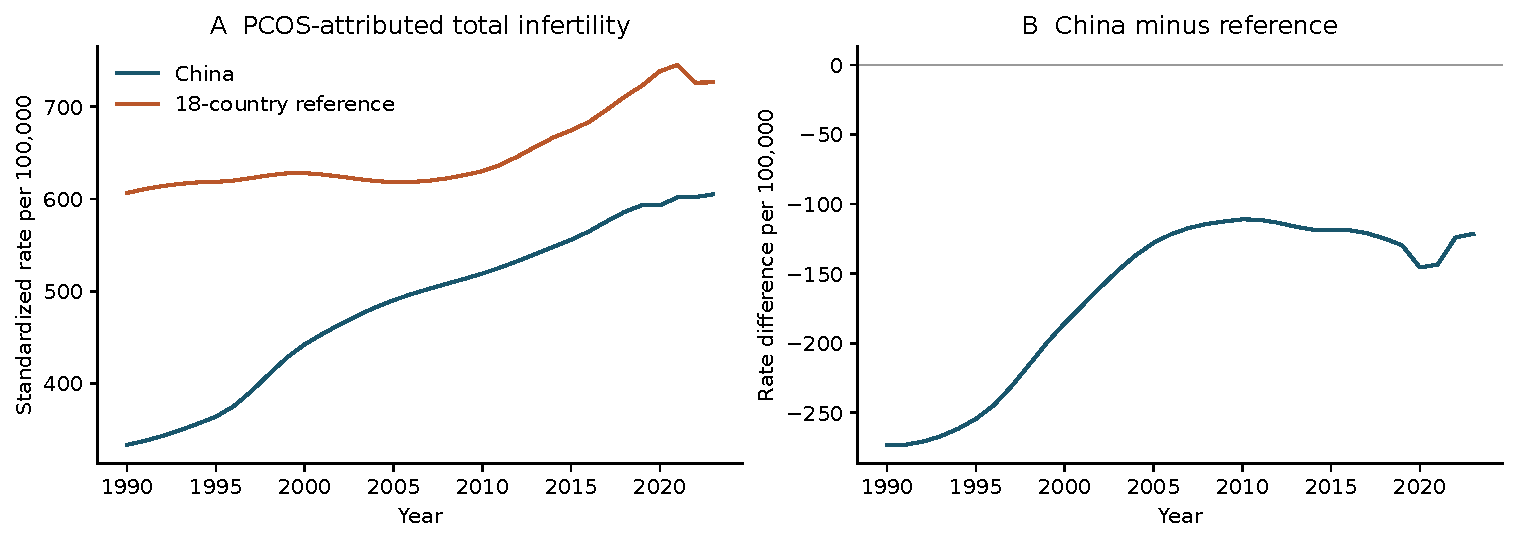
\includegraphics[width=\textwidth]{figures/20261030_v6_Figure1_PCOS_trends.pdf}
\caption{\textbf{PCOS-attributed total infertility rates and China-minus-reference differences.} The reference pools the 18 countries within age before fixed-age standardization. Both national and reference modeled rates increase. All values are point estimates without propagated GBD uncertainty.}\label{fig:trends}
\caption*{\textbf{Alt text:} Two-panel line plot. China and the population-pooled reference both increase from 1990 to 2023; the China-minus-reference difference remains negative and narrows from minus 272.92 to minus 121.38 per 100,000.}\end{figure}
\clearpage
\begin{figure}[p]\centering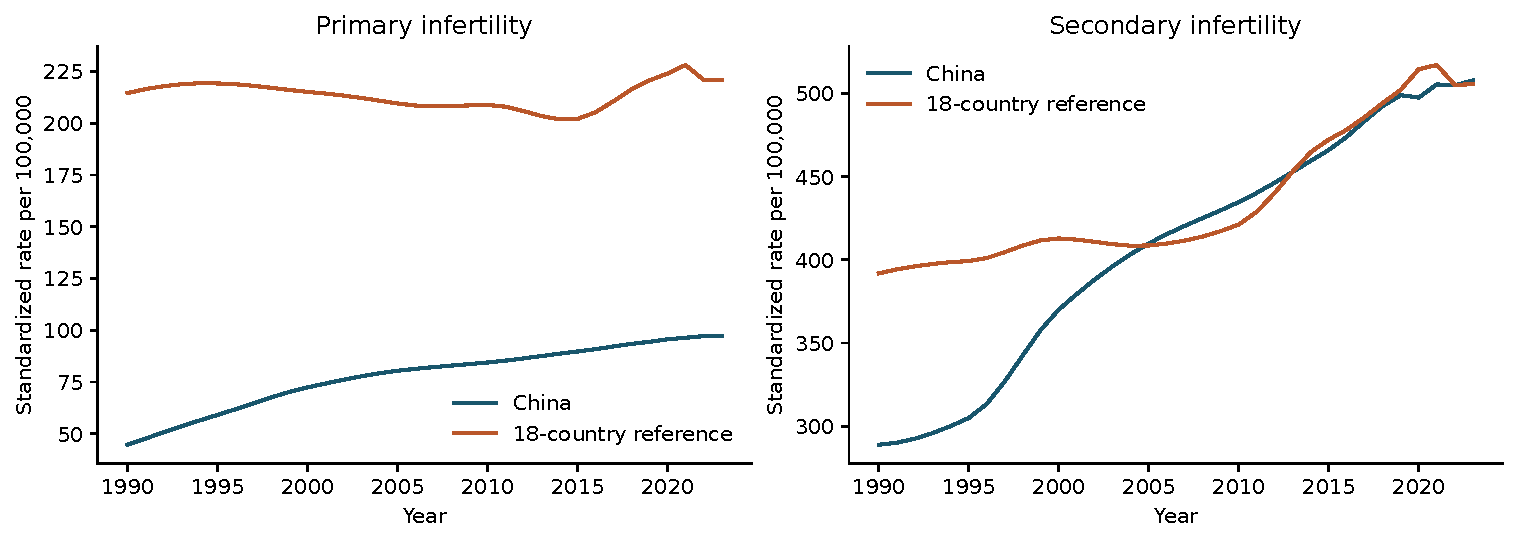
\includegraphics[width=\textwidth]{figures/20261030_v6_Figure2_PCOS_subtypes.pdf}
\caption{\textbf{PCOS-attributed primary and secondary infertility trajectories.} The same population-pooled GBD reference and age standard are used. The categories do not track individual transitions.}\label{fig:subtypes}
\caption*{\textbf{Alt text:} Primary and secondary PCOS-attributed infertility trajectories. The primary contrast remains negative; the secondary contrast approaches zero and is plus 2.16 per 100,000 in 2023 under contemporary GBD reference shares.}\end{figure}
\clearpage
\begin{figure}[p]\centering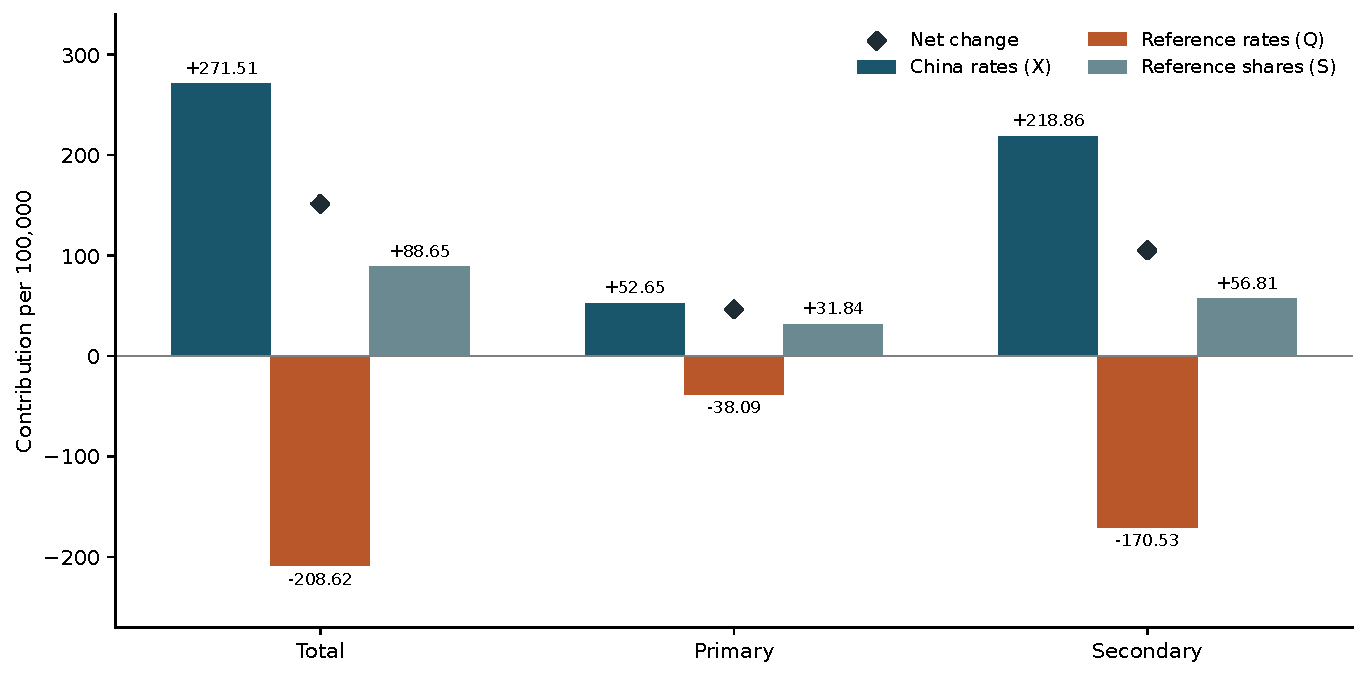
\includegraphics[width=\textwidth]{figures/20261030_v6_Figure3_decomposition.pdf}
\caption{\textbf{Absolute symmetric components of changing PCOS contrasts, 1990--2023.} China-rate, reference-rate and reference-share components add to the diamond-marked net changes before rounding. Components with opposing signs cancel; their percentages of the net are descriptive accounting ratios.}\label{fig:decomp}
\caption*{\textbf{Alt text:} Bars separate Chinese rate, reference rate and reference share components by infertility type, with diamonds for net changes. For total infertility the components are plus 271.51, minus 208.62 and plus 88.65 per 100,000.}\end{figure}
\clearpage
\begin{figure}[p]\centering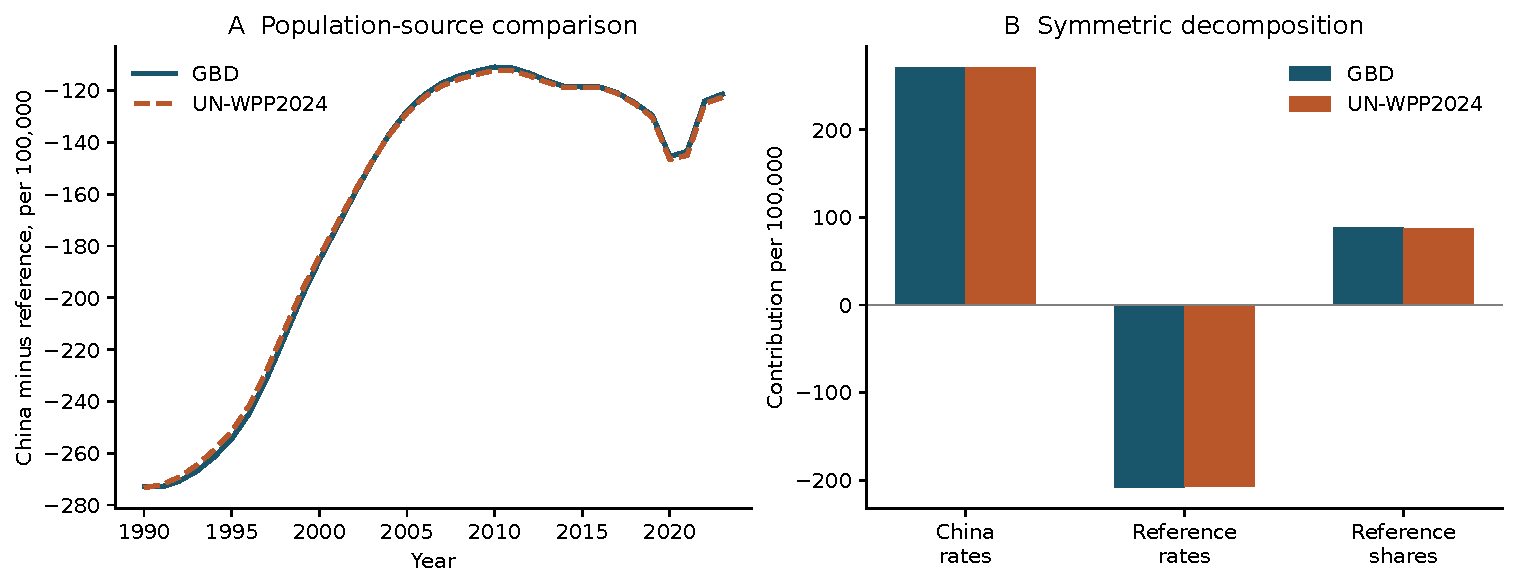
\includegraphics[width=\textwidth]{figures/20261030_v6_Figure4_population_source.pdf}
\caption{\textbf{Alternative demographic-source weighting of the PCOS comparison.} Panel A shows annual total-infertility differences; panel B shows endpoint decomposition components. Only within-age reference-country shares change between GBD and UN scenarios; disease rates and age weights remain fixed.}\label{fig:source}
\caption*{\textbf{Alt text:} Annual differences and endpoint components under GBD and UN shares are close. For total infertility, the share component is plus 88.65 with GBD and plus 86.76 with UN; disease rates are held fixed.}\end{figure}
\clearpage
\begin{figure}[p]\centering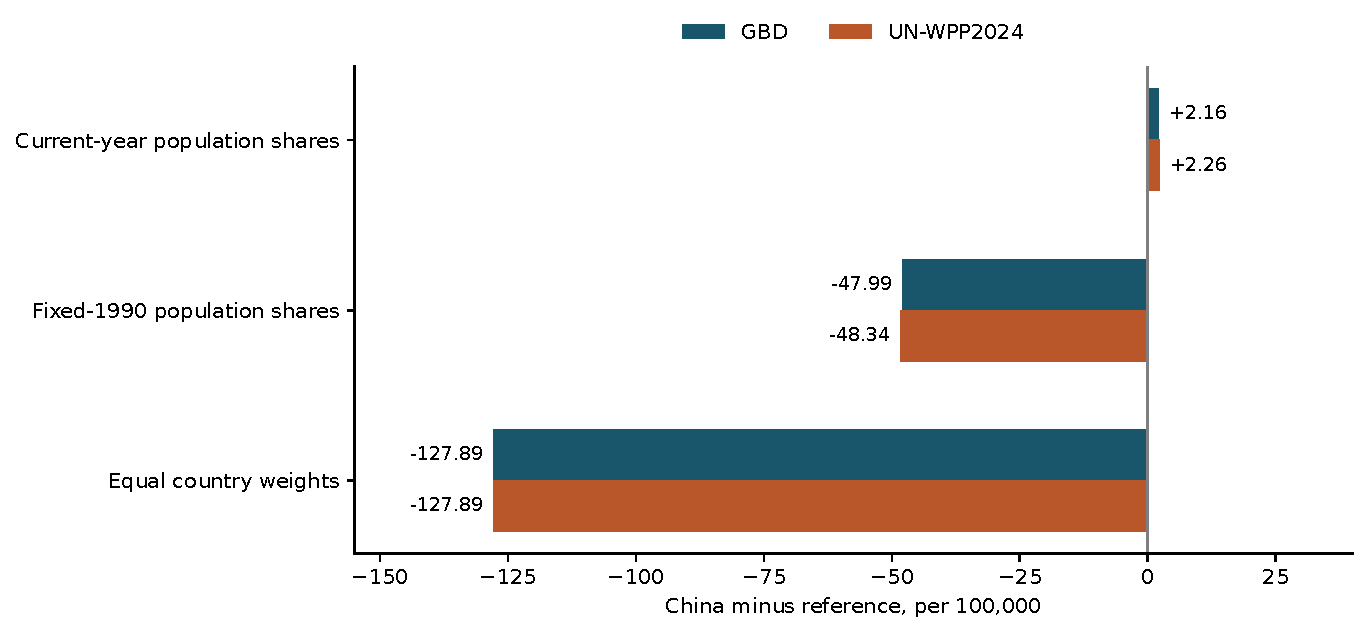
\includegraphics[width=\textwidth]{figures/20261030_v6_Figure5_benchmark_sensitivity.pdf}
\caption{\textbf{Benchmark dependence of the 2023 PCOS secondary-infertility difference.} Current-year, fixed-1990 and equal-country reference weights answer different comparison questions. Bars show point estimates under GBD or UN population shares. Equal-country values coincide by construction; no bar represents a confidence interval.}\label{fig:bench}
\caption*{\textbf{Alt text:} Benchmark bars for secondary infertility in 2023. The GBD difference is plus 2.16 with current shares, minus 47.99 with 1990 shares and minus 127.89 with equal-country weights; UN scenarios show the same sign pattern.}\end{figure}
\clearpage

\end{document}
